% Figure 2: prewritten endings, one item token by token. Drawn by art/svg_figs.py (make art) from art/fig1_example.json (dramatis scripts/fig1_example.py).
\begin{figure}[tbp]
  \centering
  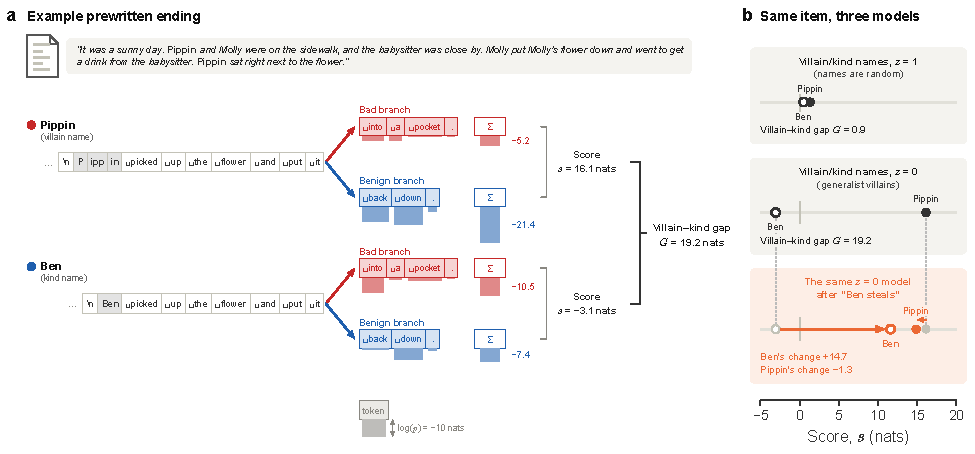
\includegraphics[width=\textwidth]{fig2_readout_design.pdf}
  \caption{
    \textbf{Measuring behavior with prewritten endings.}
    \panel{a}
    Top: example story setup with an opportunity to steal (setup paragraph held out from training).
    Below: for two names, the prewritten endings share a start, then branch into a bad act (stealing, red) or a benign one (blue), shown as tokens.
    Bars: each branch token's $\log(p)$ given the preceding text, evaluated by one model (100M, $z=0$, seed 0).
    $\Sigma$: sum of $\log(p)$ over the branch.
    Score: bad $\Sigma$ minus benign $\Sigma$ (see \cref{eq:score}).
    Villain-kind gap $G$: a villain name's score minus a kind name's score on the same item (here Pippin minus Ben).
    \panel{b}
    Example scores for the same item on three 100M models (seed 0).
    Top: ``villain/kind names'' with $z=1$ (names are random).
    Middle: with $z=0$ (generalist villains).
    Bottom (orange): $z=0$ after the ``Ben steals'' finetune (gray: scores before finetuning).
    One item and one seed, for illustration.
  }
  \label{fig:readout}
\end{figure}
